\chapter{Lyapunov exponents and chaos}

\begin{center}
\colorbox{LightBlue}{\parbox{1\textwidth}{\noindent{\bf Note:} There is no need to repeat the information provided during the guided session. Answer the questions as concise and accurate as possible. Use graphical and/or tabular presentation rather than full sentences. The \textit{page limit} for this exercise is \textit{5 printed pages}, including figures.}}
% I adapted the page limit, because of the abandoned Chau's circuit part. It was 7 previously.
\end{center}


\begin{Exercise}[name=Lyapunov exponents of the Lorenz Equations]
The \textsc{Matlab} source code for this part of the assignment will be distributed during the session. You will get the files \verb$rhs_lorenz.m$ and \verb$lyapunov.m$.  The file \verb$rhs_lorenz.m$ contains the righthand side of the famous Lorenz equations, as well as the corresponding variational
equations.  The file \verb$lyapunov.m$ contains a function that computes and plots the Lyapunov exponents; it takes as input a
function such as \verb$rhs_lorenz.m$ and a number of method parameters.

\Question Take a careful look at this code and explain how/why it computes the Lyapunov coefficients.  What do the variables \verb$st$ and
\verb$kkmax$ mean?  For the Lorenz equations, the Lyapunov exponents are approximately 0.9, 0 and -14.57. Verify this using the \textsc{Matlab} code. Experiment with the method parameters and discuss how they influence the accuracy of the obtained results.
\Question How can you interpret these results? What link can you make between Lyapounov exponents and eigenvalues of fixed points?

\end{Exercise}

\begin{Exercise}[name=The Duffing oscillator]

The Duffing oscillator with periodic forcing can be described by the following differential equation
\begin{equation}
\ddot{x}+k\dot{x}+x^3=B\cos t,
\end{equation}
in which you are asked to choose the model parameters $k$ and $B$ such that the oscillator is in a chaotic regime (see figure). Make sure not to take exactly the same parameter values as a different group. 

\Question Discuss the system behaviour and the sensitivity with respect to the initial conditions.  Illustrate your claims by making use of time plots and phase diagrams.

\Question Repeat this experiment for parameter values in the subharmonic regime and show how this case differs from the chaotic case.

\textbf{Hint: } Transform the Duffing equation to a state space representation. You can then use \textsc{Matlab}'s \verb$ode45$ solver to simulate the time behaviour. See the \textsc{Matlab} help for details.

\Question Use the code from the previous exercise to compute the Lyapunov exponents and discuss.

\vfill
\begin{center}
    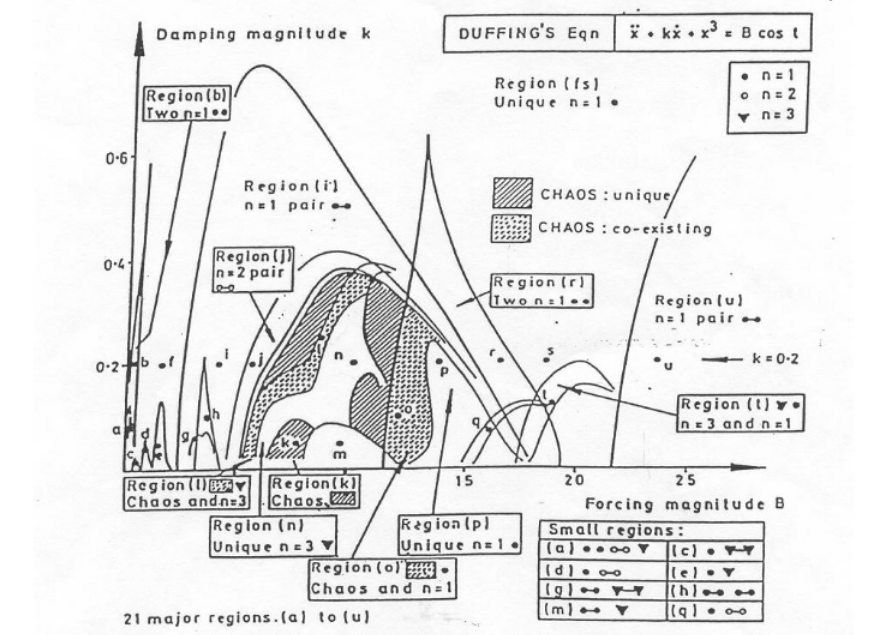
\includegraphics[width=0.85\textwidth]{duffing_bis}
    \captionof{figure}{Regimes of the various long-term behaviors of Duffing's equation\footnotemark{},\footnotemark{}}
\end{center}
\vfill

\end{Exercise}\footnotetext[1]{J. M. T. Thompson, H. B. Stewart, \emph{Nonlinear Dynamics and Chaos}, Wiley, 1986.}\footnotetext[2]{Y. Ueda, \emph{Steady motions exhibited by Duffing's equation}, IPPJ--434, 1980.}

% \begin{Exercise}[name=Chua's circuit]

% Consider the following non-linear (but piecewise linear) circuit.

% \noindent The dynamics of this circuit are given by
% \begin{equation*}
% \begin{cases}
% C_1\cfrac{\mathrm{d}v_{C_1}}{\mathrm{d} t} &= G(v_{C_2}-v_{C_1})-g(v_{C_1})\\
% C_2\cfrac{\mathrm{d}v_{C_2}}{\mathrm{d} t} &= G(v_{C_1}-v_{C_2})+i_L\\
% L\cfrac{\mathrm{d} i_L}{\mathrm{d} t} &= -v_{C_2}
% \end{cases}
% \end{equation*}
% with $g(\cdot)$ the piecewise linear characteristic that is depicted in the figure.  The parameter values are chosen to be
% \begin{displaymath}
% \begin{array}{ccccccc}
% \pj{\cfrac{1}{C_1}=11} & \pj{\cfrac{1}{C_2}=2} & \cfrac{1}{L}=7 & G=0.7 &
% m_0=-0.5 & m_1 = -0.8 & B_p = 1
% \end{array}
% \end{displaymath}

% The system can be written as
% \begin{equation*}
% \begin{cases}
% \cfrac{\mathrm{d} x}{\mathrm{d} \tau}&=\alpha(y-h(x))\\
% \cfrac{\mathrm{d} y}{\mathrm{d} \tau}&=x-y+z\\
% \cfrac{\mathrm{d} z}{\mathrm{d} \tau}&=-\beta y
% \end{cases}
% \qquad h(x)=
% \begin{cases}
% bx+a-b &  x > 1\\
% ax & |x|\le 1\\
% bx-a+b & x <- 1
% \end{cases}
% \end{equation*}
% via
% \begin{displaymath}
% \arraycolsep=8pt\def\arraystretch{2.2}
% \begin{array}{lll}
% x=\cfrac{v_{C_1}}{B_p}, & y=\cfrac{v_{C_2}}{B_p}, & z=\cfrac{i_L}{B_pG},
% \\
% \tau=\cfrac{t G}{C_2}, & a=\cfrac{m_1}{G}+1, & b=\cfrac{m_0}{G}+1, \\
% \alpha = \cfrac{C_2}{C_1}, & \beta=\cfrac{C_2}{LG^2}. &
% \end{array}
% \end{displaymath}
% \Question
% Simulate the system behaviour. Show phase portraits in $x,y$ and $z$, as well as individual trajectories starting from two sets of nearby initial conditions.  Illustrate your suspicion about the (chaotic) behaviour of the system.
% \Question
% Use the code from the previous exercise to compute the Lyapunov exponents. %It can be seen that the exponents are clearly wrong. The is caused by the discontinuous function $h$. Try to smooth the piecewise linear model, i.e. the function $h$ and calculate the Lyapunov exponents again using the same code as before.
% \vspace{2cm}
% \begin{center}
% 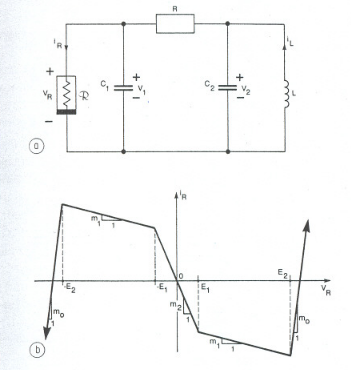
\includegraphics[width=0.55\textwidth]{chua-bis}
% \captionof{figure}{Chua's circuit, a simple autonomous circuit with a chaotic attractor\footnotemark{}.}
% \end{center}

% \end{Exercise}\footnotetext{L. O. Chua, \emph{The Genesis of Chua’s Circuit}, Archiv für Elektronik und Ubertragungstechnik, 46:250-257, 1992.}